\newcommand{\asymcloud}[2][.1]{%
\begin{scope}[#2]
\pgftransformscale{#1}%    
\pgfpathmoveto{\pgfpoint{261 pt}{115 pt}} 
  \pgfpathcurveto{\pgfqpoint{70 pt}{107 pt}}
                 {\pgfqpoint{137 pt}{291 pt}}
                 {\pgfqpoint{260 pt}{273 pt}} 
  \pgfpathcurveto{\pgfqpoint{78 pt}{382 pt}}
                 {\pgfqpoint{381 pt}{445 pt}}
                 {\pgfqpoint{412 pt}{410 pt}}
  \pgfpathcurveto{\pgfqpoint{577 pt}{587 pt}}
                 {\pgfqpoint{698 pt}{488 pt}}
                 {\pgfqpoint{685 pt}{366 pt}}
  \pgfpathcurveto{\pgfqpoint{840 pt}{192 pt}}
                 {\pgfqpoint{610 pt}{157 pt}}
                 {\pgfqpoint{610 pt}{157 pt}}
  \pgfpathcurveto{\pgfqpoint{531 pt}{39 pt}}
                 {\pgfqpoint{298 pt}{51 pt}}
                 {\pgfqpoint{261 pt}{115 pt}}
\pgfusepath{fill,stroke}         
\end{scope}}    
\newcommand{\asymcloudd}[2][.1]{%
\begin{scope}[#2]
\pgftransformscale{#1}%    
\pgfpathmoveto{\pgfpoint{321 pt}{132 pt}} 
  \pgfpathcurveto{\pgfqpoint{90 pt}{111 pt}}
                 {\pgfqpoint{127 pt}{305 pt}}
                 {\pgfqpoint{244 pt}{286 pt}} 
  \pgfpathcurveto{\pgfqpoint{59 pt}{349 pt}}
                 {\pgfqpoint{395 pt}{471 pt}}
                 {\pgfqpoint{401 pt}{423 pt}}
  \pgfpathcurveto{\pgfqpoint{512 pt}{524 pt}}
                 {\pgfqpoint{683 pt}{515 pt}}
                 {\pgfqpoint{675 pt}{376 pt}}
  \pgfpathcurveto{\pgfqpoint{852 pt}{198 pt}}
                 {\pgfqpoint{590 pt}{167 pt}}
                 {\pgfqpoint{590 pt}{147 pt}}
  \pgfpathcurveto{\pgfqpoint{481 pt}{29 pt}}
                 {\pgfqpoint{388 pt}{71 pt}}
                 {\pgfqpoint{321 pt}{132 pt}}
\pgfusepath{fill,stroke}         
\end{scope}}    

\chapter{Implementation}

In this chapter, I develop the requirements for a new random model of directed graph, 
and produce a formal definition of such a 
graph model. I present a correspondence between this model and the previous directed stochastic 
block-model that allows comparing the experimental performance of clustering algorithms between 
the two models, and provide an algorithm that efficiently samples graphs from this model. 

Next, I describe my implementations of the core clustering algorithms that have 
been developed for the purpose of recovering directional communities, and provide an insight into 
the libraries I use to implement my code-base, and lay out the structure of it. 

I furthermore give a detailed account of the set-up of my experimental analysis of the algorithms:
This involves choosing and justifying a measure for determining the quality of a resulting 
clustering, and introducing different parameterisations, the performance impacts of which will be 
interesting, that I use to critically evaluate the algorithms' performance. I also introduce ways 
that have, in the setting of undirected graphs, been used to improve the performance of clustering 
algorithms and how they might help improve performance in this setting.

\section{Heterogeneous Digraphs With Directional Communities}
\subsection{Further Requirements and Background}


A previously developed model of digraph that exhibits power-tail degree distributions was 
developed by Price \cite{price}. His original aim was to model the procedural growth of networks where new 
nodes prefer to attach to nodes with already high numbers of incoming edges. This setting of 
network formation, which extends far beyond computer networks, is of great pertinence to 
machine learning, so I decided to use the high-level technique of \emph{preferential attachment} 
to generate graphs. Formally, in Price's model, the graph grows one vertex at a time, attaching to, 
on average, $c$ other vertices, where the probability of attaching to a vertex $v$ is proportional
to $d_v + a$, where $d_v$ is the in-degree of $v$ and $a$ is some constant allowing newer vertices 
to gain incoming edges. Therefore, when the $(n+1)$th vertex is added to the graph, for each edge 
it forms, any vertex $1 \leq v \leq n$ has probability
$$
	\frac{d_v + a}{na + \sum_i d_i}
$$
of being the receiving vertex for this edge.

Now, this technique of procedural generation makes for a fundamental difference in the generation
of graphs to the stochastic block-models of before. In those models, the characteristic 
communication between clusters is enforced by choosing edge orientation after both vertices have 
been selected. However, in a model like Price's, the direction of an edge is decided by the 
relative `ages' of the two nodes; an older node may never send an edge to a newer one. This 
reflects a property of networks such as citation networks: A research paper can usually only cite 
another which has already been published. Hence, the way I would realise the directional 
communities in my model had to differ. I made the decision to make the choice of receiving 
vertex in two stages. First, one of the underlying clusters would be chosen to send the edge 
towards, then a vertex of said cluster would be chosen using preferential attachment.

This way, I could guarantee that the definition I provide in the next section would exhibit both 
necessary properties.

\subsection{Formal Definition of Heterogeneous Digraphs}
I thus define a model I will call
\emph{Directed Stochastic Block-Model with Preferential Attachment} ($\mathrm{DSBM}_\mathrm{PA}$):
\begin{definition}
\label{def:DSBMPA}
	Suppose that $c,k,N \in \mathbb{N}$, such that $k \leq N$ and $c < N$. 
	Suppose that $a \in \mathbb{R}^+$ is some constant, and that $\mathbf{p} \in [k]\rightarrow 
	[0,1]$ is a probability distribution over a set of $k$ elements. Suppose that $\mathbf{C} 
	\in [k] \times [k] \rightarrow [0,1]$ such that $\mathbf{C}(i, \cdot)$ is a probability 
	distribution over $[k]$ for any $i \in [k]$. 

	Now, consider a stochastic process $(G_i, \mathcal{C}_i)_{i = n_0}^{i=\infty}$ where 
	each $G_i$ is a directed graph with vertex set $V_i = [i]$ such that if $i \leq j$,
	$E_i \subseteq E_j$, where $n_0 \ll N$ is some small integer, $\mathcal{C}_i \in [k] 
	\rightarrow \mathcal{P}([i])$ is a partition of the vertex set of $G_i$ and $(G_{i+1}, 
	\mathcal{C}_{i+1})$ satisfies the following:
	\begin{itemize}
		\item
		the out-degree of $i+1$ in $G_{i+1}$ is $c$,
		\item
		$\forall j \in [k]\ .\ \mathbb{P}\big(\mathcal{C}_{i+1}(j) = \mathcal{C}_i(j)  
		\cup\{i+1\} \big) = \mathbf{p}(j)$,
		\item
		$\forall j,l \in [k], v \in [i]\ .\ i+1 \in \mathcal{C}_{i+1}(j) \implies $
		$$
			\mathbb{P}\left(v \in \mathcal{C}_{i+1}(l)\big|(i+1, v)\in E_{i+1}\right) 
			= \mathbf{C}(j, l)
		$$
		and
		\item
		assuming that $(i+1, v)$ is an edge in $G_{i+1}$, and assuming that $v \in 
		\mathcal{C}_{i+1}(l)$, for any $u \in \mathcal{C}_{i+1}$, 
		\begin{align}
			\mathbb{P}(u = v) = \frac{d_u^{i+1} + a}{|\mathcal{C}_{i+1}|\cdot a + 
			\sum_{w \in \mathcal{C}_{i+1}(l)} d_w^{i+1}} \label{equ:probpickedfromclust}
		\end{align} 
		where $d_u^{i+1}$ is the in-degree of $u$ in $G_{i+1}$.
	\end{itemize}

	Then, a graph $G$ with underlying communities $\{C_i\}_{i \in [k]}$ has $G \sim 
	\mathrm{DSBM}_\mathrm{PA}(N, k, c, \mathbf{p}, \mathbf{C}, a)$ if and only if $G \sim G_N$
	and $\{C_i\}_{i \in [k]} \sim \mathcal{C}_N$.
\end{definition}

This definition of the $\mathrm{DSBM}_\mathrm{PA}$ means that the clusters underlying such a graph 
are distributed in size according to $\mathbf{p}$, the cluster an edge starting in cluster $i$ is 
selected according to $\mathbf{C}(i, \cdot)$ and within a cluster, the destination vertex of any 
edge is chosen by preferential attachment.

\subsection{Correspondence With DSBM}
I have asserted that the model defined in definition \ref{def:DSBMPA} exhibits both a power-tail 
degree distribution  and directional communities, the 
interactions of which are defined by the parameter $\mathbf{C}$. 

In previous models, such as the DSBM defined in Chapter 2, directional communities were specified 
differently. The notion of `interaction' between communities that clustering 
algorithms such as DiSim and Herm try to recover is based on the balance of directions of edges 
between clusters. In order to therefore be able to fairly assess the performance of these 
algorithms, and to compare the performance for heterogeneous graphs with that for homogeneous 
graphs, a way of, given parameters to one model, a conversion to the parameters to the other is 
required.

\subsubsection{From DSBM to $\mathbf{DSBM}_\mathbf{PA}$}
Recall, the important parameter to the DSBM is the matrix $\mathcal{F}$, which specifies the 
balance in edge directions. Its other parameters are $p, q, n, k$, the significances of which are 
explained in Chapter 2. Thus, given values for these parameters, a corresponding set of 
parameters to the DSBM with preferential attachment (indicated by a tilde) can be determined as 
follows:
\begin{itemize}
	\item
	$\tilde N = k\cdot n$, $\tilde k = k$, $\tilde{\mathbf{p}}$ is the uniform distribution over 
	$[k]$.
	\item
	$\tilde c$ will be the average out-degree of vertices in the DSBM. Now, in the undirected 
	SBM, the average degree of each vertex will be $p\cdot n + (k-1)\cdot q \cdot n$. Consider
	the fact that in any directed graph, the average out-degree is equal to the average 
	in-degree, and their sum is equal to the average degree in the undirected projection of this
	digraph. Therefore, the average out-degree should be $\tilde c = \sfrac{1}{2} \cdot 
	(pn + (k-1)qn)$.
	\item
	$\tilde{\mathbf{C}}$ is more complicated to determine. \\
	To begin, recall that $\mathbf{C}_{i,j}$ (I shall use matrix notation for convenience 
	henceforth) records the probability that an edge starting in cluster $i$ goes to cluster 
	$j$. We can easily estimate this value with high probability as (number of edges going from
	$i$ to $j$) / (number of edges starting in $i$). Therefore, we may determine the value of 
	$\tilde{\mathbf{C}}$ as 
	$$
		(\tilde{\mathbf{C}})_{i,j} = \frac{q\mathcal{F}_{i,j}}{\sfrac{p}{2} + \sum_{l \neq 
		i} q\mathcal{F}_{i,l}}
	$$
	for $i \neq j$ and 
	$$
		(\tilde{\mathbf{C}})_{i,i} = \frac{p}{p + 2\sum_{l \neq 
		i} q\mathcal{F}_{i,l}}.
	$$
\end{itemize}
The value of $\tilde a$ may be arbitrary: since it controls a quality of the graph entirely 
separate from the ideas present in the DSBM, it can be chosen according to the nature of graph that
is to be modelled.

\subsubsection{From $\mathbf{DSBM}_\mathbf{PA}$ to DSBM}
The DSBM with 
preferential attachment is strictly more expressive than the original DSBM: Above, we have shown 
that for each parameterisation to the DSBM, we may derive a set of corresponding 
$\mathrm{DSBM}_\mathrm{PA}$-parameters, and by setting $a = \infty$, the distribution of degrees 
no longer follows a power-tail distribution but is uniform, like in the DSBM. Thus, since
$\mathrm{DSBM}_\mathrm{PA}$ allows the number of edges between clusters to be pariwise different, 
and allows for disparate cluster sizes, it will not in general be possible to formulate an exact 
correspondence in this direction.  

This is why in general experiments conversion in this direction should not occur, so I omit a 
correspondence in this direction here. Approximate values that ignore these issues are not hard to 
derive, however.

\subsection[Generating Graphs From $\mathrm{DSBM}_\mathrm{PA}$]{Generating Graphs From $\mathbf{DSBM}_\mathbf{PA}$}
The final consideration one has to make in working with graphs generated by this model is that of
sampling them. Ignoring for now the precise implementation details, there is of course a fairly 
straightforward way of generating graphs of this nature. However, the na\"ive method of 
calculating the probability distribution for the target vertex of each edge will become 
undesirably slow for larger graphs, meaning that a quicker and more elegant algorithm to sample 
these graphs would be beneficial. Krapivsky and Redner introduced an algorithm that 
does so for Price's original model, which yields the basis for an algorithm sampling 
$\mathrm{DSBM}_\mathrm{PA}$ \cite{redner}. 

For $\mathrm{DSBM}_\mathrm{PA}$, we can conduct the following procedure. The main difficulty is 
picking the receiving node for an edge that begins at node $i+1$ and has been decided to end in 
cluster $j$. Now, recall that for any vertex $v$ in cluster $j$, the probability of being picked 
is as in Eq.\ (\ref{equ:probpickedfromclust}). The sum of degrees in this equation is $\sum_{w} 
d_w = | \mathcal{C}(j)| \cdot \overline d$, where $\overline d$ is the average in-degree in 
cluster $j$. Now, we can estimate both of these values with high probability as
$$
	|\mathcal{C}_{i}(j)| = \mathbf{p}_j \cdot i
$$
and 
$$
	\overline d = \frac{c \sum_{l\in[k]} \mathbf{C}_{l,j}\mathbf{p}_l}{\mathbf{p}_j},
$$
respectively. Now, suppose that we pick the target vertex differently, making one of two distinct 
choices: With probability $\phi$ we choose a vertex from cluster $j$ strictly in proportion to its 
in-degree, with probability $1-\phi$ we pick a vertex uniformly at random. That is, vertex $v$ has 
the following probability of being chosen:
$$
	\phi \cdot \frac{d_v}{\sum_w d_w} + (1-\phi) \cdot \frac{1}{|\mathcal{C}_{i}(j)|} \approx
	\phi \cdot \frac{d_v}{\mathbf{p}_j i \overline d} + (1-\phi) \frac{1}{\mathbf{p}_j i}
$$	
Now, notice that we can recover the probability from Eq.\ (\ref{equ:probpickedfromclust}) by 
choosing $\phi = \overline d / (\overline d + a)$.

This implies that the algorithm presented below samples 
from the DBSM with preferential attachment. 

\begin{algorithm}
	\caption{Sampling from $\mathrm{DSBM}_\mathrm{PA}$}
\label{algorithm:sample_PA}
	\SetKwInOut{Require}{require}\SetKwInOut{Yield}{yield}
	\SetKwFunction{InitG}{initialiseG}
	\SetKwIF{WProb}{ElseIf}{Else}{with probability}{do}{else, with probability}{else}{end}
	\SetKwRepeat{Repeat}{repeat}{}
	\SetKw{Times}{times}
	\Require{Parameters $N, k, c, \mathbf{p}, \mathbf{C}, a$ for $\mathrm{DSBM}_\mathrm{PA}$}
	\Yield{$(G,  \{C_i : 1 \leq i \leq k\}) \sim \mathrm{DSBM}_\mathrm{PA}(N, k, c, \mathbf{p}, 
	\mathbf{C}, a)$}
	\BlankLine
		\tcp{Initialise $G_{n_0}, \mathcal{C}_{n_0}$ arbitrarily}
		$G , \mathcal{C}\longleftarrow$ \InitG$(k, n_0)$\;
		let $\mathtt{edges}\in\mathcal{C} \rightarrow \mathcal{P}(E(G)$ record the edges 
		that end in each cluster\;
		\For{$i = n_0+1 \hdots N$}{
			pick cluster $j$ according to $\mathbf{p}$\;
			\Repeat{$c$ \Times}{
				pick target community $l$ according to $\mathbf{C}_j$\;
				\uWProb{$\frac{\overline d}{\overline d + a}$}{
					select an edge $(u, v) \in \mathtt{edges}(\mathcal{C}(l))$ 
					uniformly at random\;
					create new edge $(i, v)$\;
				}
				\uElse{
					select a vertex $v\in \mathcal{C}(l)$ uniformly at random\;
					create a new edge $(i,v)$\;
				}
			}
			add $i$ as a node to $G$ and to $\mathcal{C}(j)$\;
			add all newly created edges to $G$\;
		}

		\KwRet{$(G, \mathcal{C})$}
\end{algorithm}

Note how picking a target node in proportional probability to its in-degree is handled by actually 
picking an edge ending in the chosen cluster uniformly at random. 

\section{Code Implementations}
\subsection{Directory Outline and Project Infrastructure}
\lstinputlisting[style=mystyle]{project_structure.txt}

The code written for this project is fairly straightforwardly organised. Auxiliary files required for the execution using Python 3 are excluded here. In general, to run experiments, the script in $\mathtt{run\_tests.py}$ is extended to cann the right functions provided by files in $\mathtt{testing/}$. Once the concepts behind each component of this testing infrastructure have been grasped, the code is not hard to understand, so I will not linger on it too much.

\subsection{Language Choice and Libraries Used}

In this section, I describe the initial decisions I made in my implementations, and give justification why these decisions were prudent and helped make my code 
more efficient and effective.

The foremost decision made, underlying all subsequent decisions in this regard was using Python 3
for implementations of clustering algorithms, random-graph generation etc. I made this decision based on a number of reasons:

\paragraph{Extensive Availability Of Pre\"existing Libraries}
Python is, of course, a very high-level programming language. For most common problem statements, 
there already exists a library implementing standard solutions in an efficient way. This directly 
harmonises with the nature of spectral clustering techniques, which themselves conduct very few 
low-level computations but instead rely on high-level subroutines such as singular-value 
decomposition or Lloyd's algorithm for $k$-means clustering. This also means that myself 
implementing these subroutines for the purpose of this project would likely have caused a 
significant loss of efficiency and would not have contributed to the validity of the project, 
rather the contrary. 

\paragraph{Efficiency} 
Though Python, in general, is not known to be a particularly fast programming language, it does 
offer tools for highly efficient computation with matrices, such as \texttt{NumPy}/\texttt{SciPy}. Since graph 
clustering, like any machine-learning task, is generally most interesting and most important for 
large inputs, the matrices in the spectral-clustering setting would otherwise provide a severe 
obstacle in this project---since the inputs to spectral-clustering algorithms are $N\times N$ 
(complex) matrices, where $N$ is the number of vertices, inefficient tools for the handling of 
these would cause severely costly run-times. 

%\paragraph{Simplicity and Similar Reasons}
%The final reasons are of a less scientific nature, though justify my choice of Python as well. 
%Firstly, Python provides a very simple and readable syntax which allows the programmer to focus 
%entirely on the content of the code, which in the case of spectral clustering techniques is not 
%trivial. Furthermore, since the algorithms discussed in this project are extremely new and 
%previously only discussed in research papers, Python's readability (which includes the ability to 
%use e.g.\ Greek letters for variable names) allows one to see the immediate correspondence between 
%the mathematical descriptions of the algorithms and the code implementation, which helps with the 
%understanding of both the code implementation and the mathematical description.
%
%More specifically, I used a number of well-known libraries implementing the high-level subroutines 
%required throughout the project. These included \texttt{NumPy} and its parent \texttt{SciPy}, as 
%well as \texttt{scikit-learn}. The subroutines required of each of these, as well as their 
%implementations' benefits are described in more detail in the relevant parts of the upcoming 
%sections; the general uses and benefits however are:

\paragraph{Code Vectorisation}
\texttt{NumPy} and \texttt{SciPy} provide an interface that allows treating vectors and matrices 
as mathematical objects rather than 1- or 2-dimensional arrays in code. This not only increases 
readability  but also dramatically improves the code's efficiency by exploiting the 
independence of single elements in vector operations, allowing the code to be executed in parallel.
\\
One particular example of this is the ability to express matrix multiplication in these libraries 
as in infix operator \texttt{@}, which not only hides the complicated implementation of matrix 
multiplication underneath but also provides highly optimised performance.

\paragraph{Professional Implementation of $k$-Means}
The \texttt{scikit-learn} implementation of Lloyd's algorithm for $k$-means clustering has several
benefits over a self-written one. Firstly, although Lloyd's algorithm in general is conceptually 
simple and straightforward to implement, there are many considerations to be made concerning edge
cases and convergence. These considerations are handled by the 
\texttt{scikit-learn} implementation using e.g.\ parallelisation to help with the performance of 
the $k$-means algorithm. Again, implementing this algorithm myself whilst taking care of these 
issues would distract from the purpose and intended focus of this project, which is why I use the
standard implementation.

\subsection{Implementing Graph-Sampling}

For both random-graph models, the code implementation of the sampling algorithm had to remember 
to generate the graph adjacency matrices in a sparse representation; this is necessitated firstly by
the need to have sparse representations in later matrix operations which would cause memory errors
when operating on dense matrices of the sizes of interest to the project. Secondly, it is made 
possible by the seamless linear-algebra implementation for sparse representations of 
\texttt{scipy.sparse}.

The second thing the implementations of both random-graph models had to satisfy was to return the
ground truth of the underlying clusters in when sampling the graph. This causes more challenge 
for one model than the other.

\subsubsection{Basic DSBM}
Sampling from the Directed Stochastic Block-Model is fairly straightforward. Since the edges are 
generated independently, and the exact number of vertices in each community is known beforehand,
one can simply generate all edges in blocks, as the name of the model suggests, which allows one 
to make use of the vectorised operations of the libraries used.

\subsubsection{DSBM With Preferential Attachment}
The sampling of graphs from $\mathrm{DSBM}_\mathrm{PA}$ is less straightforward. As Alg.\ %
\ref{algorithm:sample_PA} shows, these graphs must be generated vertex by vertex, which 
corresponds to the intial use of preferential-attachment models as procedural network-growth.
Furthermore, this view of the graph sampling means that the \texttt{SciPy} array view is no longer 
appropriate for the intermediate representation of these graphs as they are generated. Instead,
I make use of the \texttt{networkx} library which not only allows for dynamic graph modification 
but also for marking each vertex with a cluster meaning that the second requirement may still be
satisfied fairly easily. 

Obtaining the adjacency matrix for this graph in a sparse format is then also easily handled by 
\texttt{networkx}, which simply provides methods for generating the adjacency matrix of a graph.

\subsection{Implementing Spectral Clustering Methods}
\subsubsection{DiSim}
In the DiSim algorithm, recall that the crucial step delivering functionality is the construction
of the directed Laplacian, $O^{-\sfrac12} \times A \times P^{-\sfrac12}$, where $O$ and $P$ are 
matrices recording the out- and in-degrees of vertex $i$, respectively. 

Therefore, the first challenge that one encounters in the implementation of DiSim is the 
computation of this Laplacian. Here, exploiting certain properties of this construction became 
necessary. Even though the matrices $O, P$ are very sparse, calculating a sparse matrix's inverse 
square root is a very slow process which requires large quantities of memory because the inverse 
square root of a sparse matrix is not in general sparse itself. However, one may exploit that $O, P
$ are in fact diagonal matrices so calculating any power of them is achieved by performing this 
calculation element-wise on the diagonal. This makes this first step of DiSim very fast.

A second benefit of this insight is that the Laplacian is merely a scaled variant of $A$ itself, so
is sparse, and the singular-value decomposition of the matrix can be done using sparse 
linear-algebra algorithms, allowing for a far more efficient execution. At this point, it may be 
worth noting the significance of the singular-value decomposition as opposed to finding 
eigenvalues and eigenvectors. Since the Laplacian constructed by DiSim is not Hermitian, its 
eigenvalues are not in general real, so we cannot impose an ordering on them to determine which 
eigenvectors should be used for clustering. However, this complication has an advantage for the 
flexibility of the algorithm: By using the left singular vectors, the algorithm clusters vertices 
based on their `sending' behaviours, whereas clustering based on the right singular vectors allows 
clustering based on the `receiving' behaviours of the vertices. 

Then it is
merely a question of applying $k$-means to these singuar vectors to complete the algorithm, which
due to the high-level libraries available is no cause for complication.

\subsubsection{Hermitian Spectral Clustering}
Herm avoids the complication of having a non-Hermitian matrix construction
by applying the construction described in Alg.\ \ref{algorithm:herm} from Chapter 2. Thus, 
arguably, it is conceptually easier to understand, Chapter 2 also gives an explanation for \emph
{why} this construction tracks the desired information. However, working with complex numbers also 
introduces some complications for a programmer. The matrix $P$ constructed before clustering is, 
as mentioned, real due to convenient properties of $A_\mathrm{Herm}$ \cite{lucapaper}. %TODO add reference here!
However, in practice, I found that the numerical computation of the eigenvectors of 
$A_\mathrm{Herm}$ caused small imaginary parts to remain since the eigenvectors were complex-valued
and could not be calculated exactly. This difficulty had to be tackled since Lloyd's algorithm
does not cater for complex-valued data. However, an easy fix is to discard the remaining imaginary 
parts which proved to be of the order of $10^{-5}$. 

A much more significant challenge in the implementation of Herm proved to be the parameter $\epsilon$. In theory, the optimal value for this 
parameter can be established as $10 \cdot \sqrt{\tilde p \cdot \log\tilde p}$, where $\tilde p$ 
is an estimate of the parameter $p$ from the DSBM. This does not work in practice. A solution that 
does (provided $N > k$) is to take the top $k$ eigenvectors, with respect to 
eigenvalue magnitude, which in my implementation became the default approach.

\section{Experimental Set-up and Evaluation Metrics}

This section describes my approach to evaluating the performance of the clustering algorithms in 
the face of heterogeneous digraph. I first develop an argument for a measure of performance. I then discuss 
what experiments might be of interest and what expectations one might have of the development of 
performance as different parameters vary as part of each experiment. 

\subsection{Decisions about Performance Evaluation}
Evaluating the performance of these spectral clustering algorithms raises a few questions: Is the 
algorithm run-time important? Given that each algorithm attempts to recover the underlying 
community structure, how can we formalise measuring the quality of these outputs? What baseline 
should we compare these performances to?

For the purposes of this project, the question of each algorithm's run-time is of little
interest: As presented, Herm will be much slower than DiSim. This is because the matrix $P$ (the 
rows of which are subjected to Lloyd's algorithm during the execution of Herm) is of dimension $N
\times N$, meaning that the clustering proceeds over $N$-dimensional space, while in DiSim the 
clustering only occurs in $k$-dimensional space. In truth, the much more interesting question to
consider is the quality of results each algorithm obtains. 

\subsubsection{Possible Quality Measures}
As indicated above, the quality of an algorithm's output given a particular graph should be 
indicative of how well this output aligns with the underlying community structure in the graphs. 
Of course, this is not a well-defined measure, so I present two ways of formalising it. 

\paragraph{Number of Misclustered Vertices} 
One measure of alignment between the underlying communities and the clustering 
results is the minimum number of vertices that would have to be re\"assigned in the clustering 
result to recover the ground truth perfectly. Obviously, this provides a number that can easily be 
interpreted and may be scaled for presentation as a percentage. So consider a mathematical way of defining this number. Let $S_k$ be the symmetric
group on $k$, that is the set of permutations of $[k]$. Then the number of misclustered vertices may be caclulated by 
$$
	\frac12 \cdot \min_{\sigma\in S_k} \sum_{i=1}^{i=k} 
	|A_{\sigma(i)} \setminus C_i| + |C_i \setminus A_{\sigma(i)}|
$$
where the two partitions of the vertex set being compared are $A_1\hdots A_k$ and $C_1 \hdots C_k$,
and the factor of \sfrac12 has the purpose of correcting the double-counting of the misclustered 
vertices.

This measure has several serious issues. \\
Firstly, it assumes that the number of clusters in the underlying community structure is the same 
as that in the attempted solution. Secondly, this measure involves an optimisation over all 
permutations of a set, which will mean that the time it takes to compute grows factorially in $k$. 
Finally, consider a random partition of the vertex set, or one that is as `misaligned' as possible: 
Necessarily some vertices will be deemed correctly clustered by this measure. 

All of these issues are addressed by the Adjusted Rand-Index (ARI).

\paragraph{ARI} The Rand-Index takes two partitions $A_1 \hdots A_a$ and $B_1 \hdots B_b$ of a set $S$, and 
calculates the following numbers: The number of pairs of elements that are grouped together in 
both partitions, the number of pairs of elements that are not grouped together in both partitions 
and the number of pairs of elements that are grouped together in one parition but not the other.
It then divides the sum of the total 
number of pairs of elements in $S$; $\binom{|S|}{2}$. 

The ARI corrects this for chance by first calculating a `contingency table'; an $a\times b$-dimensional matrix with elements $n_{ij}\coloneqq|A_i\cap B_j|$.
Then, let $a_i \coloneqq |A_i|, b_i \coloneqq |B_i|$ and observe that if two partitions $A_1'\hdots
A_a', B_1'\hdots B_b'$ are selected at random uniformly from those such that $|A_i'|=|A_i|, |B_i'|
= |B_i|$, then it can be shown %TODO: Reference to https://link.springer.com/content/pdf/10.1007/BF01908075.pdf
that 
$$
\mathbb E\left(\sum_{i,j}\binom {n_{ij}'}{2}\right) = 
\frac{\sum_i \binom{a_i}{2} \sum_j \binom{b_j}{2}}{\binom{|S|}{2}}
$$
(where $n_{ij}' \coloneqq |A_i' \cap B_j'|$) \cite{hubert}.

From this, the ARI was developed as 
$$
	\frac{\text{agreeing pairs} - \text{expected number of agreeing pairs}}{\text{upper bound
	of agreeing pairs} - \text{expected number of agreeing pairs}}.
$$
This gives a final formula for the ARI as
$$
	\frac{\sum_{i,j} \binom{n_{ij}}2 -\frac{\sum_i\binom{a_i}2\sum_j\binom{b_j}2}{\binom{|S|}2}}
	{\frac12\left(\sum_i{\binom{a_i}2} + \sum_j\binom{b_j}2\right) - \frac{\sum_i\binom{a_i}2\sum_j\binom{b_j}2}{\binom{|S|}2}}.
$$

In the case of perfect alignment, i.e.\ identical partitions, the ARI will be 1, whilst a partition
picked randomly will yield ARI very close to 0 as the number of agreeing pairs concentrates around 
its expected value. Indeed, partitions worse than randomly picked will yield a negative ARI. This 
provides a useful, interpretable scale of values.

\subsubsection{Implementation of ARI}
It will be noticed that the task requiring the most time in the computation of the ARI is the 
construction of the contingency table. This task, if na\"ively implemented, would require 
iterating through each of the pairs of cells in the partitions and calculating their intersection. 
However, one can exploit the highly optimised implementation of matrix multiplication in \texttt
{NumPy} and other vectorised operations to reduce the time cost significantly over the na\"ive 
solution. The contingency table can in fact be calculated as $T_A \times T_B^T$, where $(T_A)_{i,j}
\coloneqq 1[j \in A_i]$, and similarly for $T_B$ (where, without loss of generality we assume the 
vertex set to be $[N]$). 

\subsection{Experiments to Be Conducted}
This section concerns the different parameters in sampling the graphs which will affect the 
performance of the clustering algorithms on the sample graphs. This firstly requires a brief discussion of 
what comparisons will be made in the experimental set-up, as well as discussing what questions 
will be interesting from a machine-learning perspective. 

\subsubsection{Establishing Baselines}
Recall that the main interest of this project is the effect of a skewed degree distribution on the clustering algorithms' performance. This is why I compare the performance of the clustering algorithms on graphs 
sampled from $\mathrm{DSBM}_\mathrm{PA}$ with the performance on graphs sampled from the DSBM  
using the correspondences established previously. The graphs sampled from the DSBM will establish a useful baseline for performance 
since they provide an almost idealised input to such directed clustering techniques, which is why 
the performance for preferential-attachment graphs should be compared against that baseline rather 
than perfect performance.

Further recall that the aim of graph clustering algorithms is, given some graph, `recover' an 
optimal graph to which noise has been added. Therefore, another point of interest is testing the development 
of performance as the adversarial noise in the graph sampling is varied. Different kinds of noise include different edge directions 
between clusters and cluster-internal edges. 

By the former, I mean that if two clusters $C_1, C_2$ `communicate' primarily through edges 
leading from $C_1$ to $C_2$, then the edges leading from $C_2$ to $C_1$ impair the `purity' of 
this balance and make the cluster interaction less clear. The second kind of noise should be more 
easily understood: If a particular vertex's edges all progress between distinct clusters and do 
not remain in one, more edges provide information about the interactions between clusters, whereas 
no such information is provided by edges connecting vertices of the same community.

The 
significance of this idea of noise is that clearly, the more such noise is present, the worse 
performance should be expected, and so a second important baseline to establish is the performance 
when there is no noise in the meta-structure of the graph. 

\subsubsection{General Meta-Graphs}
The significance of any machine-learning method is determined by the applicability of the input 
model to the real world. Thorughout this dissertation, I have mentioned the communication 
structure and `meta-graphs' as the information conveyed by a directed graph with directional 
communities. However, I have not given a concise definition of what I mean by this. 
The meta-graph of a directed graph $G$ with directional communities is the directed graph with 
vertices representing the communities in $G$, and edges between each pair of communicating 
communities in the direction of communication imbalance.

It is the meta-graph that carries the significant information in both described graph models, since
the individual vertices and edges in a paritcular instance of a meta-graph do not influence the 
overall clustering result significantly when there are tens of thousands of vertices. Therefore,
the basic performance experiments are conducted over a range of meta-graphs selected for their 
relevance to real-world networks.

\paragraph{Randomly Oriented, Complete Meta-Graphs} The first family of meta-graph I considered is
that obtained by modelling informative communication between each pair of clusters. That is, in 
a randomly oriented, complete meta-graph (ROCMG), each pair of clusters is distinguishable by the imbalance 
in edge directions between the two vertices, where the imbalance direction is decided at random. 
More specifically, such meta-graphs are generated by giving each edge in the undirected complete 
graph over the communities a direction that is decided by a fair coin-flip. 

Let me remind the reader of the parameter $\mathcal{F}$ in the DSBM, which stores in $F_{i,j}$ the
probability that an edge between clusters $i$ and $j$ goes from $i$ to $j$. For the DSBM, we may
use $\mathcal F$ to specify the meta-graph, in $\mathrm{DSBM}_\mathrm{PA}$ we would use the 
parameter $\mathbf C$. However, since we wish to compare results, we will be specifying meta-graphs 
in the DSBM and use the translation correspondence established before. So, in a noisy meta-graph 
with \emph{noise parameter} $\eta$, $\mathcal F$ is determined by $\mathcal{F}_{i,i} = \sfrac12$
for any $i$, $\forall i < j. \mathcal F_{i,j} = 1-\eta$ with probability $\sfrac12$ and otherwise
$\mathcal{F}_{i,j} = \eta$. Recall that $\mathcal F_{j,i} = 1-\mathcal{F}_{i,j}$ so the values of 
$F_{i,j}$ for $i > j$ are determined by the previously chosen values. 

ROCMGs are interesting as they provide the `easiest' input for a clustering algorithm, since
as much directional-community information as possible is included in them. With a slight 
generalisation allowing different degrees of communication imbalance, they could also be made to 
be the most general meta-graph, though in the interest of simplicity of generation, I only 
consider meta-graphs with fixed imbalances. 

\paragraph{Cycles} Cyclical meta-graphs may be used to model feedback loops in communication,
which obviously occur in many real-world scenarios and therefore present a particularly interesting
family of meta-graphs to study. Cyclical meta-graphs are more easy to explain, and define: In the
DSBM, the parameter $\mathcal F$ takes values $\mathcal{F}_{i, i\oplus 1} = 1-\eta$, where $\oplus$
denotes addition modulo $k$. For all pairs $i,j$ such that $\mathcal 
F_{i,j}$ is not determined by this rule, there is no informative communication imbalance and so 
$\mathcal F_{i,j} = \sfrac12$ for these pairs of clusters. However, this is where a weakness in the
DSBM is highlighted; after all the number of edges between any two clusters will be the same, 
determined by the parameter $q$, and so a cyclical meta-graph in the DSBM would in truth look like 
the one presented in Fig.\ \ref{fig:cycmeta}. It is immediately visually clear that not only will
a large number of noisy edges persist in this model, but the realism of this meta-graph might be 
questioned considering the kind of networks it should model. 


\begin{figure}
\floatbox[{\capbeside\thisfloatsetup{capbesideposition={right,center},capbesidewidth=.5\textwidth}}]{figure}[\FBwidth]
{
\caption{A cyclical meta-graph on five clusters as used in the DSBM. Arrow direction indicates 
communication, arrow weight indicates frequency of edge direction.}
\label{fig:cycmeta}
}{
\begin{tikzpicture}
\node[draw, circle, minimum size=1cm] (c1) at (0:2cm)   {};
\node[draw, circle, minimum size=1cm] (c2) at (72:2cm)  {};
\node[draw, circle, minimum size=1cm] (c3) at (144:2cm) {};
\node[draw, circle, minimum size=1cm] (c4) at (216:2cm) {};
\node[draw, circle, minimum size=1cm] (c5) at (288:2cm) {};
\draw[line width=2pt, -{Latex[length=3mm, width=3mm]} ] (c1) -- (c2);
\draw[line width=1pt, -{Latex[length=3mm, width=1.5mm]} ] (c1) edge[out=144, in=18, bend right=10] (c3);
\draw[line width=1pt, -{Latex[length=3mm, width=1.5mm]} ] (c1) edge[out=198, in=0, bend right=10] (c4);
\draw[line width=2pt, -{Latex[length=3mm, width=3mm]} ] (c2) -- (c3);
\draw[line width=1pt, -{Latex[length=3mm, width=1.5mm]} ] (c2) edge[out=216, in=54, bend right=10] (c4);
\draw[line width=1pt, -{Latex[length=3mm, width=1.5mm]} ] (c2) edge[out=288, in=90, bend right=10] (c5);
\draw[line width=2pt, -{Latex[length=3mm, width=3mm]} ] (c3) -- (c4);
\draw[line width=1pt, -{Latex[length=3mm, width=1.5mm]} ] (c3) edge[out=0, in=162, bend right=10] (c1);
\draw[line width=1pt, -{Latex[length=3mm, width=1.5mm]} ] (c3) edge[out=324, in=100, bend right=10] (c5);
\draw[line width=2pt, -{Latex[length=3mm, width=3mm]} ] (c4) -- (c5);
\draw[line width=1pt, -{Latex[length=3mm, width=1.5mm]} ] (c4) edge[out=342, in=216, bend right=10] (c1);
\draw[line width=1pt, -{Latex[length=3mm, width=1.5mm]} ] (c4) edge[out=36, in=234, bend right=10] (c2);
\draw[line width=2pt, -{Latex[length=3mm, width=3mm]} ] (c5) -- (c1);
\draw[line width=1pt, -{Latex[length=3mm, width=1.5mm]} ] (c5) edge[out=72, in=216, bend right=10] (c2);
\draw[line width=1pt, -{Latex[length=3mm, width=1.5mm]} ] (c5) edge[out=126, in=342, bend right=10] (c3);
\end{tikzpicture}
}
\end{figure}

\subsubsection{$\mathbf{DSBM}_\mathbf{PA}$-Specific Meta-Graphs}
These issues can be avoided in the more expressive $\mathrm{DSBM}_\mathrm{PA}$. Clearly, we can 
specify meta-graphs using $\mathbf C$ such that two clusters do not share any edges at all, which
will solve the model-appropriateness concern above, and the presence of inherently uninformative 
edges. Specifying an improved cyclical meta-graph using $\mathbf C$ is clearly not hard, either:
Given noise 
parameter $\eta$, we achieve this by setting $\mathbf C_{i,i\oplus 1} = 1-\eta$ and for all 
remaining $j$, $\mathbf{C}_{i,j} = \sfrac\eta {k-1}$.

A second meta-graph to which we gain access using these benefits is a tree-like structure, which 
can model many kinds of networks in which information is gathered and transported to a centralised 
processing cluster (the root of the tree). Restricting the branching factor of these trees to 2 
for the purposes of this 
project, I considered binary trees with $2^h-1$ nodes, for some integer $h$. However, caution must 
be taken in these meta-graphs, since in an entirely noise-free setting, where both children of a 
cluster $C$ send all their edges to $C$, the two clusters become statistically indistinguishable
and  recovering the underlying communities becomes impossible. Therefore, some clusters must send 
edges to clusters except their parent in order to make these clusters uniquely identifiable. 
The easiest way of guaranteeing this property is one of the two children of $C$ sending some 
proportion $\sigma$ of its edges to its sibling instead of its parent.

\subsection{Regularisation Techniques and Improving Performance}
In this section I describe two techniques used for `graph regularisation' in undirected graphs,
i.e.\ modifications made to the adjacency matrix of the input graph for spectral clustering 
algorithms that aim to counteract a skew in the degree distribution. Subsequently, I discuss what 
limitations there are to applying these techniques to directed graphs and how they may be adapted 
for this alternative setting. 

Finally, I describe a modification to Herm which may be of use in improving performance
as well.

\subsubsection{Self-Loops}
Both techniques I will describe introduce weighted edges to the graph that will change the 
degree-distribution such that it is not as skewed as before. The first technique is to introduce 
a weighted self-loop to each node in the graph, as in \cite{selfloops}. %TODO: add reference to self-loop paper
Each such self-loop will be of a weight $\tau\cdot c$, where $c$ is the average in-degree of the graph. 

The benefit of this technique in a directed setting is that the inter-cluster communication of 
the graph's vertices is not changed by this technique and if the reasonable assumption that the
graphs under consideration are simple (i.e.\ do not initially contain self-loops) is made, the newly 
introduced edges do not `interefere' with any true edges. Since these self-loops do not affect the spectra of any constructuions on $A$, they can just be simulated by shifting any calculated degree-values.

\subsubsection{Graph-Densification}
Empirically, it has been observed that in heterogeneous graphs, spectral clustering methods often 
return clusters with very unbalanced sizes, which results from small, peripheral subgraphs being only very 
sparsely connected to the rest of the graph \cite{binyureg}.  %TODO: Insert reference to that one paper
A schematic indicating such a partition is presented in Fig.\ \ref{fig:pericut}.
One way of counteracting this phenomenon is to add to the adjacency matrix a weighted version of 
the complete graph; that is, to add to the adjacency matrix $A$ the matrix $C$ with values $C_{ij} 
= \omega$ for some constant $\omega$. This makes the graph more dense, and effectively reduces the 
number of small subgraphs that are sparsely connected to the graph, meaning that cuts through 
larger components of the graph are promoted through this technique and undesirable partitions like 
the ones in Fig.\ \ref{fig:pericut} are avoided.

Here, an issue of directionality arises when trying to apply this technique to the setting of 
directed graphs. Clearly, simply directly applying this technique will cause issues in
Herm, since the crucial assumption that the modified adjacency matrix is Hermitian which underlies
the entire algorithm would be violated. Furthermore, briefly inspecting the construction 
$A_\mathrm{Herm}$ from Herm reveals a further assumption this algorithm makes about the input 
graph $G$: If $(u,v)$ is an edge in $G$, then $(v,u)$ is not. Superpositioning the complete graph
in this way would clearly violate this assumption. However, this issue might be addressed by 
orienting each edge in the superpositioned complete graph randomly with direction probability 
\sfrac12 either way, which would fix the issues discussed above. 

With both these techniques, it will be of interest to see whether they also improve the 
performance of spectral clustering algorithms in directed settings and what values will be effective.

\subsubsection{Interpolating Between Undirected and Directed Communities}
Many real-world networks do not only exhibit communities specified by their interactions. Often,
if not most of the time, communities also exhibit internal communication thus conveying information.
Clearly, this is an issue considering the foregoing discussion of community-internal edges as 
`noise'. 

However, the construction $A_\mathrm{Herm}$ used in the Hermitian algorithm need only satisfy the 
condition that it is Hermitian. Therefore, we may investigate the possibility that using values of 
$r \pm \imath$ to indicate edges, for some values $r\in \mathbb R$ would lead 
the algorithm to 
`interpolate' the clustering between the optimal directional communities and the optimal undirected 
communities, yielding applicability to use cases in which neither purely directed nor purely 
undirected clustering apply entirely. Obviously, the choice of parameters $r$ for this 
technique is linked to the number of edges within clusters, so this relation has been 
investigated as well.

\begin{figure}
\floatbox[{\capbeside\thisfloatsetup{capbesideposition={right,center},capbesidewidth=.31\textwidth}}]{figure}[\FBwidth]
{
\caption{Often, sparsely connected peripheral subgraphs lead to poor partitions, when ones with more edges (as indicated in the dotted line) would be preferable.}
\label{fig:pericut}
}{
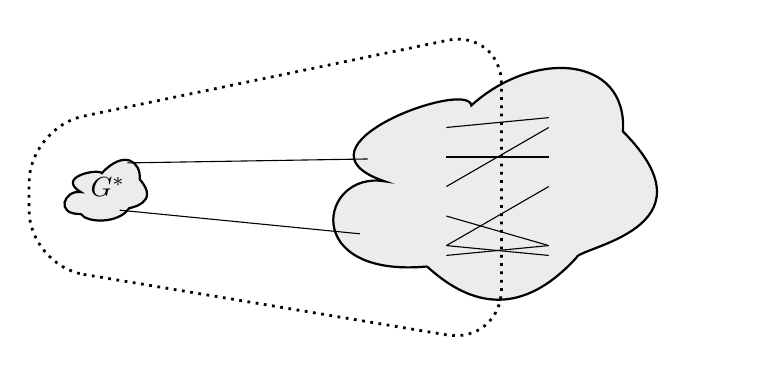
\begin{tikzpicture}
\node (gsc) at (0,0) {\tikz\asymcloud[.05]{fill=gray!15, thick};};
\node (gsl) at (0,0) {$\scriptsize{G^*}$};
\node (gpc) at (5,0) {\tikz\asymcloudd[.2]{fill=gray!15, thick};};
\draw (0.25, 0.3) -- (3.3,0.35);
\draw (0.15, -0.3) -- (3.2, -0.6);
\draw (4.3, -.75) -- (5.6,0);
\draw (4.3,-0.375) -- (5.6,-.75);
\draw (4.3,0) -- (5.6,.75);
\draw (4.3,0.375) -- (5.6,0.375);
\draw (4.3,-.875) -- (5.6, -.75);
\draw (4.3,.75) -- (5.6,.875);
\draw (4.3,-.75) -- (5.6,-.875);
\draw[line width=1pt, dotted, rounded corners=20] (-1, -1) -- (5,-2) -- (5, 2) -- (-1, .75) -- cycle;
\end{tikzpicture}
}
\end{figure}
